\documentclass{beamer}
\mode<presentation>
{
  \usetheme{myulm}
  \setbeamercovered{transparent}
  \setbeamertemplate{navigation symbols}{} % no navigation bar
  \setbeamersize{sidebar width left=1.17cm}
}

\usepackage[ngerman]{babel}
\usepackage[utf8]{inputenc}
\usepackage{amsmath,amssymb,amsfonts}
\usepackage{times}
\usepackage{graphicx}
\usepackage{fancyvrb}
\usepackage{array}
\usepackage{colortbl}

% Anfang der Titelfolie
% Anpassung von: Titel, Untertitel, Autor, Datum und Institut

\title{Kanonische Transformationen und die Hamilton-Jacobi-Gleichung}
\subtitle{Seminar I für Computationals Science and Engineering bei Prof. Lebiedz}
\author{Alexander Dürr und Anton Hügel}
\newcommand{\presdatum}{8. Februar 2018} % alternativ zu \today: Eingabe eines festen Datums
\institute
{\\Universität Ulm, Institut für Numerische Mathematik}
%Ende der Titelfolie

% Anfang der Kopfzeile der Folien
% Anpassung von: Zwischentitel, Leitthema oder Name
% Das Datum wird oben geändert: unter \presdatum{}!

\newcommand{\zwischentitel}{Zwischentitel}
\newcommand{\leitthema}{Lanczos Kap. 7 und 8}
% Ende der Kopfzeile

% Anfang der Folien
\begin{document}
\hspace*{-1.49cm}
\frame[plain]{\titlepage}

% Das Inhaltsverzeichnis
\hspace*{-0.7cm}
\begin{frame}
  \frametitle{Inhaltsverzeichnis}
  \tableofcontents
\end{frame}


\section{Bekanntes: Die kanonischen Gleichungen}

\section{Kanonische Transformationen}
    \begin{frame}
    \frametitle{Gesucht: Lösung der kanonischen Gleichungen}
    
    \begin{align*}
        \dot{q}_k &= \frac{\partial H}{\partial p_k} \\
        \dot{p}_k &= -\frac{\partial H}{\partial q_k}
    \end{align*}
    
    
\end{frame}

    \subsection{Lösung mechanischer Probleme mittels Koordinatentranformation}
    \begin{frame}
    \frametitle{Ausweg: Koordinatentransformation}
    
    Gesucht wird ein Koordinatensystem, indem die kanonischen Gleichungen direkt gelöst werden können.
    
    \begin{figure}
        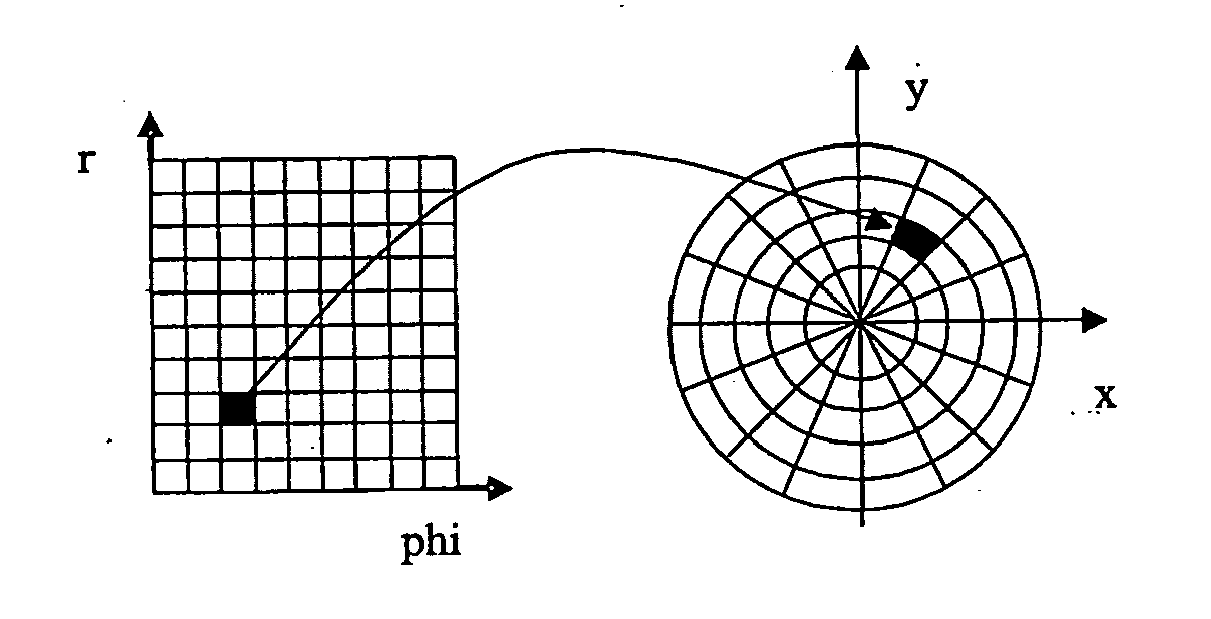
\includegraphics[scale=0.2]{images/koordtrans.png}
    \end{figure}
    
    
\end{frame}

\begin{frame}
    \frametitle{Ausweg: Koordinatentransformation}
    
    \textbf{Wichtig:} Lösungen müssen erhalten bleiben.\\
    D.h. wir brauchen Transformationen, gegenüber derer die kanonischen Gleichungen invariant sind. \\
    \vspace{5mm}    
    Solche Transformationen werden \emph{kanonische Transformationen} genannt.
    
    \begin{figure}
        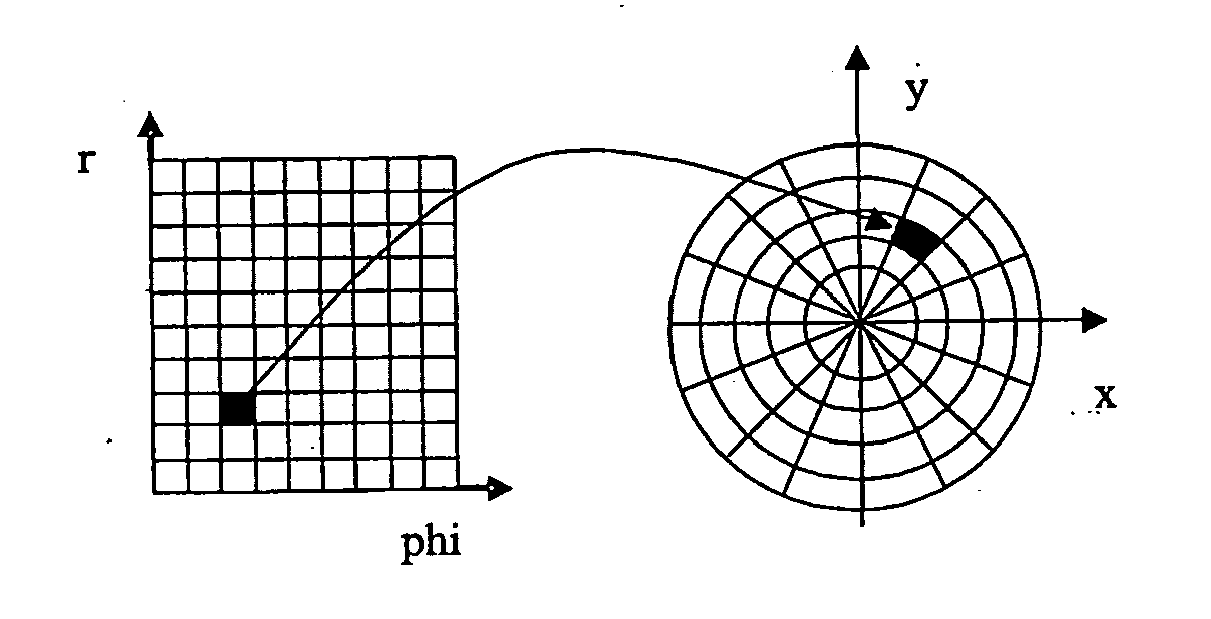
\includegraphics[scale=0.2]{images/koordtrans.png}
    \end{figure}
    
    
\end{frame}
    
    \subsection{Die Langrange'sche Punkttransformation}
    \begin{frame}
    \frametitle{Punkttransformation}
    
    Alte Koordinaten: $p_k, q_k$ \\
    Neue Koordinaten: $P_k, Q_k$
    
    Punkttransformationen haben die Form
    
    \begin{align*}
    q_1 &= f_1(Q_1,\ldots,Q_n) \\
        &\quad\vdots \\
    q_n &= f_n(Q_1,\ldots,Q_n)    
    \end{align*}
    
\end{frame}


    
    \subsection{Die allgemeine kanonische Transformation}
    
    \subsection{Die Bilineare Differentialform}
    
    \subsection{Infinitesimale kanonische Transformationen}
    
    \subsection{Das Phasenfluid als kanonische Transformationen}
    
    
\section{Die Hamilton-Jacobi-Gleichung}

    \subsection{Jacobis Transformationstheorie}
    
    \subsection{Lösung durch Separation}
    
    \subsection{Partielle Differenzialgleichungen bei Hamilton und Jacobi}

    \subsection{Geometrische Lösung und Wellenanalogie}

\section{Zusammenfassung}


\end{document}